\chapter[SCP-105 “鸢娓”]{
    SCP-105 “鸢娓”\\
    SCP-105 "Iris"
}

\label{chap:SCP-105}

\begin{figure}[H]
    \centering
    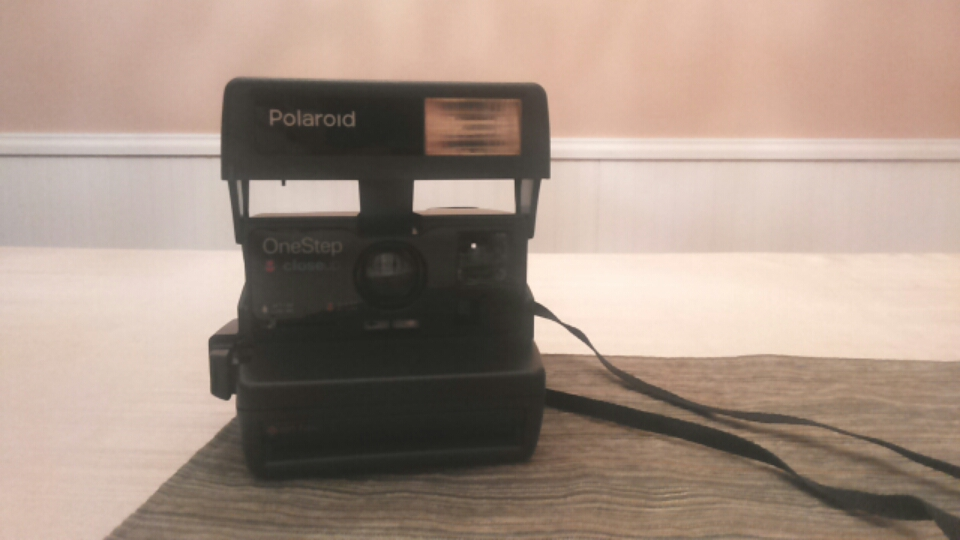
\includegraphics[width=0.5\linewidth]{images/SCP.105.jpg}
    \caption*{SCP-105-B}
\end{figure}

\bb{项目编号:}SCP-105

\bb{项目等级:}Safe

\bb{特殊收容措施:}SCP-105现居于Site-17并被植入追踪装置。SCP-105现时获准与受认证的Site成员进行三级(受限)特许社交接触,建基于其持续的良好行为及与基金会人员合作的前提下授予。

SCP-105的个人相机(指定为SCP-105-B)被存放于Site-19高价值物品储藏设施的保险箱里。标准主动防御措施(爆炸,生化及模因)应根据标准作业措施随时待命。

在未经多数O5议会投票批准下,SCP-105及SCP-105-B的接触是不被允许的。

\bb{描述:}SCP-105(原名 Iris Thompson)是一名欧裔女性。 记录指出SCP-105出生于████,推算出对象在被收容时年龄为██岁。她拥有金发蓝眼,现高1.54米,重50kg。她没有表现出任何异常的物理特性,总言而之,是一名健康的正常人类。

SCP-105-B是一台1982年出产的Polaroid One Step 600相机\footnote{\bb{译注:}Polaroid是一所著名的拍立得相机品牌,它的相机拍完照可以立即冲洒出来。}。SCP-105-B没有表现出任何异常的物理特性,总言而之,被SCP-105以外的人员操作时是一台普通的拍立得相机。

当SCP-105持有由SCP-105-B拍下的照片时,照片会从静止图像转变为该拍摄地点的实时影像。SCP-105亦能穿过照片并从拍摄位置操纵照片范围内的物件。上述操作的目击者报告指他们看见一只无实体的女性手掌(后确认为SCP-105)从一个看不见的传送门伸出并进行上述行为。SCP-105-B以及它所拍下的照片被其他人使用时并没表现出不寻常的特性。

SCP-105已展示了透过其他照片操纵物件的能力,但表示在使用SCP-105-B时是最顺手的。

\bb{附录1:收容时的情况:}SCP-105于她男友被谋杀后不久引起基金会注意。SCP-105声称当她男友被杀的时候她正在跟他通电话,促使她赶至他的所在地;但是,电话记录与她的叙述不符,使她成为此谋杀案的最大嫌疑者。 SCP-105随后告诉她的律师,事实上她是透过前些日子和她男友的合照看到他被杀害的。该律师无视该辩词并建议对方承认控罪。对象拒绝认罪,后来因一级谋杀罪罪名成立而被判死刑。

对象从死囚中被招募,并立即转移至特殊收容措施(Special Containment Procedures)以待确认她的能力。基金会人员从SCP-105的家中回收SCP-105-B(以相同型号替换),并归还给她。进一步的测试证实了SCP-105的能力,随后它被移至Site-17,命名为SCP-105。

\bb{附录2:摘自访谈记录105-08-4426,于██\slash ██\slash ████}

\begin{scpbox}

\bb{<记录开始>}

\ii{Dr. █████:}请进行一段自我介绍,包括出生日期及地点,还有妳的名字。

\ii{SCP-105:}好的…我的名字是Iris Thompson,于████年五月十二日,在亚利桑那州凤凰城出生。

\ii{Dr. █████:}很好。第一条问题,妳是什么时候察觉到你有这样的能力呢?

\ii{SCP-105:}我不太肯定,不过我想大慨是在十到十一岁左右。我记得当时我看著一张海洋的照片,然后我发现里面的波浪开始动起来。

\ii{Dr. █████:}当你告诉你家长这件事的时候他们有什么反应?

\ii{SCP-105:}他们只告诉我我想太多了。

\ii{Dr. █████:}那你是什么时候发现你能透过照片操纵物件呢?

\ii{SCP-105:}那时我十二岁。在我的家人带我去大峡谷旅游之后,我正翻看著相簿,然后我不小心碰到照片里的一颗在崖上的小石头并推动了它。 最初我以为这是我的幻想,但之后我就成为了一名摄影爱好者。我到处留影。但要不是在我十三岁的时候,我父母送了我一台拍立得相机,我通常都不能对它们做些什么。我很喜欢那台相机因为我觉得它让事情易办多了。

\ii{Dr. █████:}那就是我们称为105-B的相机?你的私人相机?

\ii{SCP-105:}是的,长官。

\ii{Dr. █████:}你一次能注视多少张照片?

\ii{SCP-105:}我曾试过一次十张照片,但我觉得我能做的更好。

\ii{Dr. █████:}你在对于在基金会中的这段长时间的印象如何?

<SCP-105一言不发。>

\ii{Dr. █████:}请你回答。我们不会对此而见怪于你的。

\ii{SCP-105:}就类似于…新的囚牢,新的狱卒。但我知道这比原来将发生在我身上的事要好点。

\ii{Dr. █████:}你在这里的一段时间里都很合作。

\ii{SCP-105:}我是那类很守规矩的人。我也喜欢做那些实验。那些我从未想像过的东西的照片也是。

\ii{Dr. █████:}Iris,你知道为什么我问你这些问题吗?

\ii{SCP-105:} 我不知道,长官。

\ii{Dr. █████:}我们正进行一个特殊计划。如果一切顺利,你就能离开站点前往外边的世界。而我们只需要你一点点的帮助。你有与趣吗?

\bb{<记录结束>}

\end{scpbox}

\bb{附录3:于MTF Omega-7的服役史:}

\ii{Iris是第二名被主动吸收进MTF Omega-7,潘多拉之盒的人员。不同于负责攻坚行动的Able小队(和\hyperref[chap:SCP-076]{SCP-076}-2有关),Iris小队主要负责侦察及情报收集任务。Iris小队和Bowe委员会合作完成超过二十个任务,从所有迹象看,这些任务皆迅速完成而没有发生任何事故。}

\ii{首宗SCP-105被牵涉在内的纪律事故涉及一次把由Iris小队负责的侦察任务升级至湿活\footnote{\bb{译注:}原文wetwork,代指杀人等会沾血的脏活。}的指令。SCP-105坚拒使用她的能力进行暗杀行动,即使Bowe委员会的成员重复试图寻求她的合作亦是如此(详见访谈记录105-21-6543)。}

\ii{在此次事件中,SCP-105变得情绪低下并企图欺骗基金会人员使其相信她的异常特性已经消失。D███████博士提文报告建议将SCP-105重编级为Neutralized,在进行记忆消除后,放归到社会中持续监视。此建议被拒绝了。}

\ii{在此之后,D███████博士在一次收容失效中协助SCP-105逃离基金会的羁押。此次失效以失败告终,SCP-105亦被重新收容(详见事故X45-Site-17)。}

\ii{事后访谈证实D███████博士刻意鼓励SCP-105声称失去异常能力。SCP-105重新展示她的能力,作为交换,她有限度的权限被恢复。}

\ii{随著潘多拉之盒计划被终止,所有的MTF Omega-7小队被解散,而SCP-105则回到Site-17里。因她带来的安全风险,她现时不允许接触SCP-105-B。}

\ii{所有有关MTF Omega-7的资讯根据记录及资讯安全行政部(Records And Information Security Administration)的命令已被封存。}

\ii{██████ ███主管,记录及资讯安全行政部}

\bb{附录4:特别注意事项,RE:当前信息限制状态}

\ii{在\hyperref[chap:TALE-immediate-actions]{事故R1300-Site-17}之后,很多关于SCP-105及假想其与\hyperref[chap:COMP-resurrection]{MTF Alpha-9}有联系的正式或非正式报告被提出。}

\ii{这些报告对安全产生了严重威胁。所有关于MTF Alpha-9的信息获取已被限制。所有关于当前对SCP-105异常性质进行的研究的信息获取已被限制。最近和当前所有关于将SCP-105视为基金会资产的报告和传闻被视为绝对虚假,并应上报给记录及资讯安全行政部。}

\ii{██████ ███主管,记录及资讯安全行政部}
